\documentclass[./main.tex]{subfiles}
\begin{document}


Mediante el diálogo entre los resultados experimentales, el análisis de datos y la teoría, en los capítulos anteriores logramos desarrollar una descripción conceptual de la dinámica de activación de ERK en células madre embrionarias. En esta descripción, interpretamos la dinámica de activación de ERK como oscilaciones intermitentes, con transiciones entre intervalos oscilatorios, de silencio y pulsos aislados. 

%Creemos que las oscilaciones están controladas por la dosis de FGF4, que además controla cuánto duran los intervalos oscilatorios. Tanto la duración de pulsos como el intervalo de interpulsado poseen escalas temporales similares, que parecen conservarse ante distintas dosis de estímulo extracelular. 


Observamos también que las poblaciones de ESCs presentaron una mezcla de células con dinámica puramente oscilatoria y puramente no oscilatoria, así como células que transitaban entre estos regímenes dinámicos. Este comportamiento nos sugiere que el sistema de transducción de señales FGF/ERK en ESCs se encuentra cerca de un punto de transición entre un estado no oscilatorio y uno oscilatorio. %En este marco, suponemos que el aumento de los niveles de FGF4 acercaría el sistema a este punto. En este escenario, el estado no oscilatorio podría provenir de un régimen excitable que produce pulsos aislados. 


%En este escenario, los pulsos aislados podrían ser el resultado de breves excursiones desde el régimen estacionario al oscilatorio. Alternativamente, el estado no oscilatorio podría ser un régimen dinámico distinto que produce pulsos aislados. La naturaleza del estado no oscilatorio es aún desconocida en las ESC, junto con el tipo de transición.


Buscamos resumir estas ideas en un modelo matemático de baja dimensionalidad. En este capítulo comenzamos por estudiar los regímenes dinámicos de un modelo de fase con bifurcación de ciclo infinito, e introducimos conceptos básicos de dinámica no lineal que utilizaremos en el resto del trabajo. Luego, estudiaremos cómo dependen sus principales propiedades dinámicas de los parámetros del modelo para entender la capacidad y limitaciones que éste tiene para describir la dinámica de actividad de ERK.


\section{Modelo de fase con bifurcación de ciclo infinito}
%\sectionmark{Oscilaciones y excitabilidad en un modelo de fase ...}
%\section{Oscilaciones y excitabilidad en un modelo de fase con bifurcación de ciclo infinito}
%\sectionmark{Oscilaciones y excitabilidad en un modelo de fase ...}
\label{C5_sec:osc_exc}

Buscamos una descripción de baja dimensionalidad de la dinámica de actividad de ERK. Como la relación entre la amplitud de la señal adquirida del sensor de traslocación y la actividad dinámica de ERK es desconocida, no fue posible caracterizar la amplitud de las series temporales de actividad de ERK a partir de nuestros experimentos, y decidimos no incorporar este aspecto en la teoría por el momento. Elegimos describir el estado dinámico del sistema con una variable angular o fase, e interpretaremos como pulsos de ERK a los ciclos de la fase. En este marco, optamos por comenzar a trabajar con un sistema dinámico que tiene la capacidad de dar lugar a oscilaciones y silencios, que son regímenes dinámicos que observamos en las series temporales experimentales. 

Para presentar este sistema dinámico, nos enfocaremos en describir las propiedades dinámica de una fase $\theta(t)$ cuya dinámica esté descripta por la ecuación de Adler \cite{Strogatz1994}
\marginpar{ecuación de Adler}
\begin{equation}
    \dot{\theta}(t) = \omega + \alpha \sin{(\theta(t))},
    \label{C5_eq:adler_determinista}
\end{equation}
donde en esta notación $\dot{\theta}(t) \equiv \frac{d\theta(t)}{dt}$ es la velocidad de la fase $\theta(t)$. La ecuación \ref{C5_eq:adler_determinista} tiene dos parámetros $\alpha$ y $\omega$, cuyas unidades son de $\frac{1}{\text{tiempo}}$. Para introducir cómo es la dinámica gobernada por esta ecuación, comenzaremos por describir cómo es la evolución temporal de $\theta(t)$ a medida que cambiamos el parámetro $\alpha$, dejando fijo $\omega$. Por simplicidad, trabajaremos con valores no negativos de los parámetros.

\marginpar{frecuencia del\\uniforme}
Cuando $\alpha = 0$, la ecuación \ref{C5_eq:adler_determinista} describe la dinámica de un oscilador uniforme de frecuencia $\omega$. Invocando esta propiedad, llamaremos a $\omega$ la \textbf{frecuencia del caso uniforme}. 


Para estudiar los casos en que $\alpha \neq 0$, es útil visualizar el diagrama de fases de la ecuación \ref{C5_eq:adler_determinista}.\marginpar{diagrama de fases} En el contexto de dinámica no lineal, un diagrama de fases es un plano de coordenadas cuyos ejes son dos variables de estado, por ejemplo $\dot{\theta}(t) $ y $\theta(t)$. En el plano se dibujan posibles soluciones del sistema de ecuaciones diferenciales que gobiernan la dinámica del sistema, como por ejemplo la ecuación \ref{C5_eq:adler_determinista}. El sistema dinámico $\theta(t)$ se mueve a lo largo de estas trayectorias a medida que trascurre el tiempo, a partir de su condición inicial. Analizando las soluciones representadas en el diagrama de fases, es posible obtener un análisis cualitativo de la dinámica que representa.


En la figura \ref{C5_fig:adler_determinista_oscilatorio}A observamos el diagrama de fases de la ecuación \ref{C5_eq:adler_determinista} para el caso en que $\alpha$ es positivo y pequeño en relación a $\omega$. Observamos en este diagrama que\marginpar{amplitud de\\modulación} la \textbf{amplitud de modulación} $\alpha$ introduce una no-uniformidad en el flujo alrededor del círculo. Es decir, la velocidad del sistema dinámico-representada en el eje y-no es igual para todos los valores de $\theta$-representados en el eje x-. En particular, a partir del gráfico \ref{C5_fig:adler_determinista_oscilatorio}A podemos deducir que el flujo es más rápido cuando $\theta = \frac{\pi}{2}$, el máximo del seno, y más lento cuando $\theta = \frac{3 \pi}{2}$, el mínimo del seno. Como las velocidades máximas y mínimas dependen de la suma y la diferencia entre la frecuencia del uniforme $\omega$ y la amplitud de modulación $\alpha$, esta no-uniformidad se vuelve más pronunciada a medida que aumenta la amplitud de la modulación $\alpha$. 


\begin{figure}
    \centering
    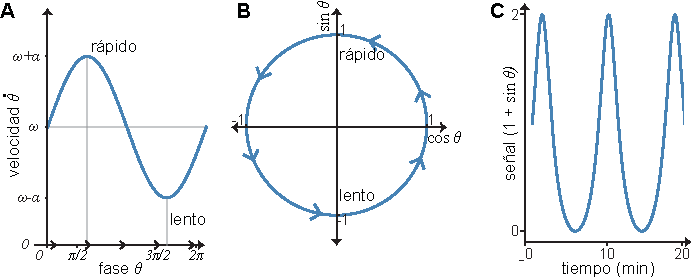
\includegraphics[width=1\columnwidth]{figures/chapter5/C5_determinista_oscilatorio.pdf} 
    \caption{\textbf{Oscilaciones no-uniformes en un modelo de fase con bifurcación de ciclo infinito.} (A) Velocidad de la fase en función de su posición entre $0$ y $2\pi$. El campo de velocidades de $\xx(t)$ también se encuentra indicado con flechas negras sobre el eje $x$. (B) Trayectoria de la fase en la circunferencia trigonométrica. El campo de velocidades de $\xx(t)$ también se encuentra indicado en la circunferencia unitaria con flechas azules. (C) Observable en función del tiempo, definido según la ecuación \ref{C5_eq:seno_fase}. La condición inicial es $\theta(0)= 0$. (A-C) Está representado el caso de oscilaciones no-uniformes de la ecuación \ref{C5_eq:adler_determinista}, donde $\omega > \alpha > 0$. Parámetros: $\alpha = 0.5 \times \omega$ y $\omega = \frac{2 \pi}{7}$. (A,B) Se encuentran indicadas las regiones de máxima y mínima velocidad.}
    \label{C5_fig:adler_determinista_oscilatorio}
\end{figure}


Gracias a la periodicidad del sistema dinámico que estudiamos, otra forma de visualizar este efecto es con la circunferencia trigonométrica de radio unidad.\marginpar{circunferencia\\trigonométrica} En esta representación, el eje x corresponde al $\cos{(\theta)}$, el eje y corresponde al $\sin{(\theta)}$, y se dibujan en el plano posibles trayectorias de $\theta(t)$. Por ejemplo, $\theta = 0$ corresponde a las coordenadas $x=1, \; y=0$, ó $\theta = \frac{\pi}{2}$ a $x=0, \; y=1$. Por ende, si $\theta(t)$ toma valores de $0$ a $10\pi$, $\theta(0) = 0$ y su velocidad es positiva y constante, en la circunferencia trigonométrica visualizaremos un círculo de radio uno y el sistema dinámico lo recorrerá en sentido antihorario comenzando en la coordenada $(1,0)$ y con velocidad constante hasta alcanzar la coordenada $(1,0)$ luego de completar $5$ vueltas. En la figura \ref{C5_fig:adler_determinista_oscilatorio}B representamos la circunferencia trigonométrica de radio unidad asociada a la dinámica representada en \ref{C5_fig:adler_determinista_oscilatorio}A. En este caso, la velocidad con que la fase recorre la circunferencia trigonométrica es positiva, pero no es constante, y depende de la localización de la fase $\theta(t)$ en la circunferencia. Las regiones de mayor y menor velocidad de $\theta(t)$ están indicadas. 


Pero, ¿cómo potencialmente se relacionaría este sistema dinámico que estamos estudiando con la actividad dinámica de ERK? Previamente establecimos que interpretaríamos un ciclo de la fase $\theta(t)$ como un pulso de actividad de ERK. Entonces, podríamos proponer como observable de la actividad de ERK cualquier función periódica de la fase, de período $2\pi$. De esta manera, la dinámica de activación de ERK estaría gobernada por la fase $\theta(t)$ y este observable representaría la señal de la dinámica de activación de ERK. Esta distinción entre fase y señal explota el hecho de que es más sencillo escribir ecuaciones diferenciales simples que determinen la dinámica del sistema utilizando la variable angular $\theta(t)$ en lugar de cualquiera de sus posibles observables, y que la señal traduce esa dinámica en series temporales que son más fáciles de visualizar e interpretar que la evolución temporal de la fase. A modo ilustrativo, podemos, por ejemplo, proponer representar a la señal adquirida de la actividad dinámica de ERK $s(t)$ como el seno de la fase $\theta(t)$ en función del tiempo. Este observable tiene la ventaja de ser la proyección de la fase $\theta(t)$ en el eje $y$ de la circunferencia trigonométrica. Para trabajar con valores positivos en la señal, proponemos \marginpar{señal de actividad de ERK}
\begin{equation}
    s(t) = 1+\sin{\theta(t)}.
    \label{C5_eq:seno_fase}
\end{equation}
Con esta definición, la señal de la dinámica representada en \ref{C5_fig:adler_determinista_oscilatorio}A,B se vería como en la figura \ref{C5_fig:adler_determinista_oscilatorio}C. En esta dinámica, vimos que la velocidad de la fase no era uniforme, y la zona de velocidades más rápidas era la región alrededor de $\frac{\pi}{2}$. En esta zona el seno tiene su máximo, y en la señal $s(t)$ la no-uniformidad se traduce en picos más estrechos comparados con oscilaciones uniformes. Por otro lado, la zona de velocidades más lentas alrededor de $\theta = \frac{3 \pi}{2}$ conduce a valles más anchos en la señal. 


Hasta ahora, consideramos el sistema dinámico de la ecuación \ref{C5_eq:adler_determinista} para el caso en donde $\alpha$ es positivo y pequeño comparado con $\omega$. Cuando el valor de $\alpha$ se acerca al valor de $\omega$, $\omega - \alpha$ se vuelve cada vez más pequeño, el mínimo del diagrama de fases \ref{C5_fig:adler_determinista_oscilatorio}A se arrimar al eje $x$, y la velocidad mínima de la fase $\theta(t)$ se acerca a $0$. En el caso límite donde $\alpha = \omega$, el mínimo del diagrama de fases de \ref{C5_fig:adler_determinista_oscilatorio}A toca al eje $x$, y la velocidad mínima de la fase $\theta(t)$ es $0$. Esto significa que cuando la fase se encuentre en este punto, permanecerá en este punto el resto del tiempo. En otras palabras, el sistema dinámico \emph{deja de oscilar} en $\theta = \frac{3 \pi}{2}$.


En el caso donde $\alpha > \omega$, la velocidad de la fase cruza dos veces el eje $x$ en \xxe y \xxi (figura \ref{C5_fig:adler_determinista_excitable}A). Además, toma valores negativos en los valores de $\theta$ comprendidos entre \xxe y \xxi. Esto significa que si el sistema se encuentra en cualquier lugar del intervalo $(\xxe,\xxi)$, la fase evolucionará con velocidad negativa hasta llegar a \xxe. De manera equivalente, si el sistema se encuentra en cualquier lugar del intervalo de velocidades positivas $(\xxi,\xxe)$, la fase también evolucionará hasta llegar a \xxe. Por esta característica de sumidero que adquiere \xxe cuando $\alpha > \omega$, se clasifica a \xxe como un punto fijo estable. Representamos al punto fijo estable como un círculo relleno en la figura \ref{C5_fig:adler_determinista_excitable}A. Por el contrario, si el sistema se encuentra en \xxi, el sistema permanecerá en \xxi. Pero siempre que el sistema esté en la vecindad de \xxi (o en cualquier otro lado), el sistema tiende a escapar de \xxi hacia \xxe.\marginpar{puntos fijos\\estables e\\inestables} Por esta característica de fuente que adquiere \xxi cuando $\alpha > \omega$, se clasifica a \xxi como un punto fijo inestable. Representamos al punto fijo inestable como un círculo vacío en la figura \ref{C5_fig:adler_determinista_excitable}A.


 \begin{figure}
    \centering
    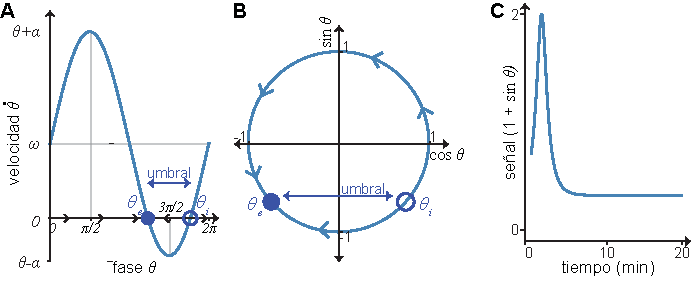
\includegraphics[width=1\columnwidth]{figures/chapter5/C5_determinista_excitable.pdf} 
    \caption{\textbf{Silencios en un modelo de fase con bifurcación de ciclo infinito.} (A) Velocidad de la fase en función de su posición entre $0$ y $2\pi$. El campo de velocidades de $\xx(t)$ también se encuentra indicado con flechas negras sobre el eje $x$. (B) Trayectoria de la fase en la circunferencia trigonométrica. El campo de velocidades de $\xx(t)$ también se encuentra indicado en la circunferencia unitaria con flechas azules. (C) Observable en función del tiempo, definido según la ecuación \ref{C5_eq:seno_fase}. La condición inicial es $\theta(0) = 6$. (A-C) Está representado el caso excitable de la ecuación \ref{C5_eq:adler_determinista}, donde $ 0 < \omega < \alpha$. En este caso, $\alpha = 1.1 \times \omega$ y $\omega = \frac{2 \pi}{7}$. (A,B) Se encuentran indicados los puntos fijos estable \xxe e inestable \xxi, y el umbral de excitabilidad.}
    \label{C5_fig:adler_determinista_excitable}
\end{figure}


Podemos determinar la localización de los puntos fijos analíticamente calculando dónde la velocidad de fase de la ecuación \ref{C5_eq:adler_determinista} se anula. Sea $\xx_f$ un punto fijo. Por su definición,  
\begin{align}
    &\partial_t \theta (\xx_f) = 0 = \omega + \alpha \sin{\xx_f}\\
    &\xx_{f1} = -\arcsin{\frac{\omega}{\alpha}} + 2 n_1 \pi \quad \text{y} \quad
     \xx_{f2} = \pi + \arcsin{\frac{\omega}{\alpha}} + 2 n_2  \pi \quad n_1,n_2 \in \mathbb{Z}.
    \label{C5_eq:PF_def}
\end{align}
En las figuras \ref{C5_fig:adler_determinista_excitable}A,B están representados los puntos fijos del intervalo $[0,2\pi)$, donde $n_1 = 1$ y $n_2 = 0$. \xxi es el punto fijo inestable, pues $\partial_t \theta (\xxi+\epsilon) > 0$ y $\partial_t \theta (\xxi-\epsilon) < 0$ para $\epsilon$ positivo y pequeño, características de un punto fuente. En cambio, \xxe es el punto fijo estable, pues $\partial_t \theta (\xxi+\epsilon) < 0$ y $\partial_t \theta (\xxi-\epsilon) > 0$, características de sumidero.


Podemos visualizar este régimen dinámico distinto en la circunferencia trigonométrica \ref{C5_fig:adler_determinista_excitable}B. Para cualquier condición inicial en $(\xxi,\xxe)$, el sistema recorrerá la circunferencia en sentido horario hasta alcanzar \xxe, y si la condición inicial del sistema es en $(\xxe,\xxi)$, el sistema recorrerá la circunferencia en sentido antihorario hacia \xxe. Ilustramos un ejemplo de la señal que adquiriríamos en este caso en la figura \ref{C5_fig:adler_determinista_excitable}C. 


En conclusión, aumentando el valor de $\alpha$ desde $\alpha < \omega$ hacia $\alpha > \omega$ aparecen un punto fijo estable y uno inestable. Esta bifurcación se conoce como bifurcación de \textit{saddle-node} de ciclo infinito\marginpar{bifurcación de\\\textit{saddle-node}\\de ciclo infinito}. 


Volvamos al régimen donde $\alpha > \omega$, e imaginemos que el sistema se encuentra en el punto fijo estable \xxe. Dadas sus propiedades de sumidero, si el sistema recibe una pequeña perturbación, rápidamente retornará hacia su estado inicial en \xxe. En la señal  del sistema, esto se traducirá como una perturbación de baja amplitud en la señal (ecuación \ref{C5_eq:seno_fase}). En cambio, si la perturbación es suficientemente grande tal que el sistema es capaz de sobrepasar el punto fijo inestable \xxi, el sistema realizará una excursión recorriendo gran parte de la circunferencia trigonométrica antes de regresar a su estado inicial en \xxe. En la señal  del sistema, esto se traducirá como un pulso. Esta característica es propia de sistemas dinámicos excitables.\marginpar{sistema dinámico\\excitable} 

Es fácil ver que la magnitud de la perturbación, o valor umbral, necesaria para realizar una excursión en el régimen excitable es la distancia angular entre el punto fijo estable y el inestable.\marginpar{umbral de\\excitabilidad} Para nuestro problema,
\begin{align}
    |\xxe - \xxi| &= |(\pi + \arcsin{\frac{\omega}{\alpha}}) -  (-\arcsin{\frac{\omega}{\alpha}})| \\
    &= |\pi + 2 \arcsin{\frac{\omega}{\alpha}}|.
    \label{C5_eq:umbral}
\end{align}
Luego, el umbral para realizar una excursión en el régimen excitable depende del cociente adimensional $\frac{\omega}{\alpha}$. 


En resumen, la ecuación \ref{C5_eq:adler_determinista} describe la dinámica de una fase de un sistema dinámico con un régimen oscilatorio cuando $\alpha < \omega$, y uno excitable cuando $\alpha > \omega$. En el régimen excitable, cuando perturbamos al sistema con un valor mayor al umbral de la ecuación \ref{C5_eq:umbral}, el sistema realiza una excursión, y en la serie temporal se visualiza un pulso (ecuación \ref{C5_eq:seno_fase}). Si los ciclos de $\theta$ representaran pulsos de actividad de ERK, los ciclos del régimen oscilatorio representarían oscilaciones de pERK. Por otro lado, una excursión en el régimen excitable representaría un pulso de actividad de ERK, con la posibilidad de ser un pulso aislado.


El modelo de fase de \ref{C5_eq:adler_determinista} es capaz de reproducir los diferentes regímenes dinámicos observados en las oscilaciones intermitentes de actividad de ERK. Sin embargo, una característica distintiva de la dinámica de activación de ERK es que la duración de sus pulsos es invariante ante transiciones entre estos distintos regímenes dinámicos, y desconocemos si esta característica es también propia del sistema dinámico que estudiamos en esta sección. A continuación, estudiaremos la duración de un ciclo de la fase gobernada por la Ecuación de Adler  \ref{C5_eq:adler_determinista} en el régimen oscilatorio, donde las oscilaciones son mayoritariamente no uniformes. Luego, estudiaremos la duración de un ciclo en el régimen excitable. 






\section{Conclusiones y discusión}


Creemos que la dinámica de activación de ERK consiste en oscilaciones intermitentes, con transiciones entre intervalos de silencio, oscilatorios y pulsos aislados. Las poblaciones de ESCs presentaron una mezcla de células con dinámica puramente oscilatoria y puramente no oscilatoria, así como células que transitaban entre estos regímenes dinámicos. Este comportamiento nos sugiere que el sistema de transducción de señales FGF/ERK en ESCs se encuentra cerca de un punto de transición entre un estado no oscilatorio y uno oscilatorio. En este marco, suponemos que el aumento de los niveles de FGF4 acercaría el sistema a este punto. En este escenario, el estado no oscilatorio podría provenir de un régimen excitable que produce pulsos aislados \cite{Lindner2004}. Buscamos resumir estas ideas en un modelo matemático de baja dimensionalidad.



La vía de señalización de ERK regula múltiples funciones celulares en diversos tipos celulares. Los principales mecanismos implicados en la activación de la vía ERK han sido bien caracterizados, y su regulación es altamente compleja (capítulo \ref{ch1}). Un modelo que contemple los componentes e interacciones de esta red resulta interesante, y ayudaría a entender cuál es origen de la dinámica de activación de ERK y las oscilaciones intermitentes. Por otro lado, desarrollar una descripción de baja dimensionalidad de la dinámica de activación de ERK en ESCs nos daría información para comprender cuál es el mecanismo dinámico que promueve esta activación. Además, nos permitiría entender cuáles son las propiedades dinámicas propias del tipo celular, y cuáles de estas características codifican información relevante para tomar decisiones de destino celular. Asimismo, una descripción de baja dimensionalidad de la dinámica de activación de ERK en ESCs es interesante desde el enfoque puramente teórico. La activación de ERK representa un tipo de dinámica previamente no descripta, y desarrollar una descripción teórica así como entender sus principales propiedades dinámicas es un aporte interesante. 


Como la relación entre la amplitud de la señal adquirida del sensor de traslocación y la actividad dinámica de ERK es desconocida, no fue posible caracterizar la amplitud de las series temporales de actividad de ERK a partir de nuestros experimentos, y decidimos no enfocarnos en describir este aspecto. Elegimos describir el estado dinámico del sistema con una variable angular o fase, e interpretaremos como pulsos de ERK a los ciclos de la fase, , y la señal de actividad según la ecuación \ref{C5_eq:seno_fase}.  En este capítulo estudiamos los regímenes dinámicos de un modelo de fase con bifurcación de ciclo infinito, cuya forma normal está descripta por la ecuación \ref{C5_eq:adler_determinista}.  Esta ecuación tiene sólo dos parámetros: la frecuencia del caso uniforme y la amplitud de modulación. Vimos que es posible transicionar entre un régimen oscilatorio y uno excitable, y la forma de atravesar la bifurcación es variando la relación entre los parámetros del modelo. 


Observamos que el régimen oscilatorio es \emph{no-uniforme} (figura \ref{C5_fig:adler_determinista_oscilatorio}), y la \emph{no-uniformidad} crece con la amplitud de modulación. Logramos reproducir la duración de pulsos para el régimen oscilatorio \cite{Strogatz1994} (ecuación \ref{C5_eq:T_osc}). Observamos que la duración de pulsos aumenta conforme al aumento del cociente adimensional entre los parámetros del modelo, y cuando disminuye la frecuencia del uniforme. Este comportamiento evidencia que aumentando la no-uniformidad de la dinámica, disminuye la velocidad mínima y aumenta la velocidad máxima que puede tener la fase. Entonces, el sistema pasa cada vez más tiempo cerca de la región de velocidades mínimas, y menos en la de velocidades máximas. Esto conduce a un aumento en la duración de los pulsos.


En el régimen excitable, aparecen un punto fijo inestable y un punto fijo estable. Su distancia depende del cociente entre los parámetros del modelo, y el sistema tiende a permanecer en el punto fijo estable (figura \ref{C5_fig:adler_determinista_excitable}). Cuando al sistema se le aplica una perturbación mayor al umbral de excitabilidad,es decir, la distancia entre los puntos fijos, la fase presenta un ciclo y la señal, un pulso. Con la perturbación, la fase sobrepasará el punto fijo inestable y hará una excursión antes de regresar al punto fijo estable. Propusimos definir a un pulso en el régimen excitable cuando el sistema sobrepasa el punto fijo inestable y realiza una excursión hacia el punto fijo estable siguiente, y definimos la duración de un pulso como el tiempo que tarda el sistema en llegar al punto fijo estable, habiendo partido del inestable (ecuación \ref{C5_eq:T_osc_def}, figura \ref{C5_fig:T_exc_def}). Con esta definición, el tiempo entre pulsos diverge, pues el sistema tarda \emph{infinito} tiempo en salir del punto fijo inestable, e \emph{infinito} tiempo en llegar al punto fijo estable. Propusimos salvar esa divergencia realizando la integral en un entorno de los puntos fijos (ecuación \ref{C5_eq:T_exc_def_eps}, figuras \ref{C5_fig:T_exc_T1},\ref{C5_fig:T_exc_T2},\ref{C5_fig:T_exc_T3}). 


Logramos calcular la duración de pulsos para el régimen excitable (expresión \ref{C5_eq:T_exc}, figura \ref{C5_fig:T_exc_res}), que coincide con nuestras mediciones en series temporales sintéticos. Observamos que la duración de los pulsos en el régimen excitable se reduce conforme aumenta el cociente entre los parámetros del modelo. Aumentando este cociente, las velocidades positivas que gobiernan las trayectorias del sistema dinámico crecen, y la reducción de la duración de pulsos es simplemente consecuencia de que el sistema dinámico se mueve más rápido desde el punto fijo inestable hacia el estable. La duración de pulsos del régimen excitable es el producto de dos factores: una expresión análoga a la duración de pulsos para el régimen oscilatorio, y un factor que depende del cociente de los parámetros del modelo y de la medida del entorno de los puntos fijos que usamos para integrar (expresión \ref{C5_eq:T_exc_aprox}). Esto sugiere una relación entre la duración de pulsos para el caso oscilatorio y el excitable. Que parte de la diferencia entre estas dos duraciones provenga de que se recorre menos trayectoria angular en un pulso no es claro, pues para la misma frecuencia del estacionario, la rapidez con que el sistema excitable recorre la circunferencia unidad es, en promedio, mayor que la del oscilatorio. Por otro lado, es probable que parte de esta diferencia se explique con la necesidad de perturbar al sistema para pulsar en el excitable. 


En resumen, estos resultados demuestran que la forma normal propuesta tiene la capacidad de transicionar entre un régimen oscilatorio y uno excitable. Por otro lado, tiene la limitación de que la duración de pulsos varía durante estas transiciones. Para continuar, es necesario evaluar si esta propiedad podría potencialmente representar parte de la variabilidad que observamos en los datos experimentales, o si es necesario modificar el modelo dinámico para que tenga capacidad de reproducir ese aspecto de las observaciones. Otra limitación que surge es que es necesario perturbar al sistema en el régimen excitable para obtener pulsos en la señal. Esta propiedad sugiere que es necesario redefinir el modelo para tener la capacidad de tener pulsos en el régimen excitable \cite{Lindner2004}. 




% ---------------------------------------------------------------------------
% --------------------------- comments --------------------------------------
% ---------------------------------------------------------------------------

%cuando lo haga, decir que las simulaciones de las TS las hice con el mismo que el que tiene ruido pero D = 0


%Creemos que las oscilaciones están controladas por la dosis de FGF4, quien además controla la duración de los intervalos oscilatorios. Tanto la duración de pulsos como el intervalo de interpulsado poseen escalas temporales similares, que parecen conservarse ante distintas dosis de estímulo extracelular.  


%En este escenario, los pulsos aislados podrían ser el resultado de breves excursiones desde el régimen estacionario al oscilatorio. Alternativamente, el estado no oscilatorio podría ser un régimen dinámico distinto que produce pulsos aislados. La naturaleza del estado no oscilatorio es aún desconocida en las ESC, junto con el tipo de transición.


%Como continuación, buscamos resumir estas ideas en un modelo matemático de baja dimensionalidad. En este capítulo comenzamos por estudiar los regímenes dinámicos de un modelo de fase con bifurcación de ciclo infinito e introducimos conceptos básicos de dinámica no lineal que utilizaremos en el resto del trabajo. Luego, estudiaremos cómo dependen sus principales propiedades dinámicas de los parámetros del modelo para entender la capacidad y limitaciones que éste tiene para describir la dinámica de actividad de ERK.


\end{document}